\section{Gesteuerter Gleichrichter}
\subsection{M1C}
\vspace{-0.5cm}
\begin{minipage}{0.4\linewidth}
    \includegraphics[width=0.8\linewidth]{images/GRM1c}
\end{minipage}
\begin{minipage}{0.35\linewidth}
    \centering %BESSERE GRAFIK EINFèGEN
    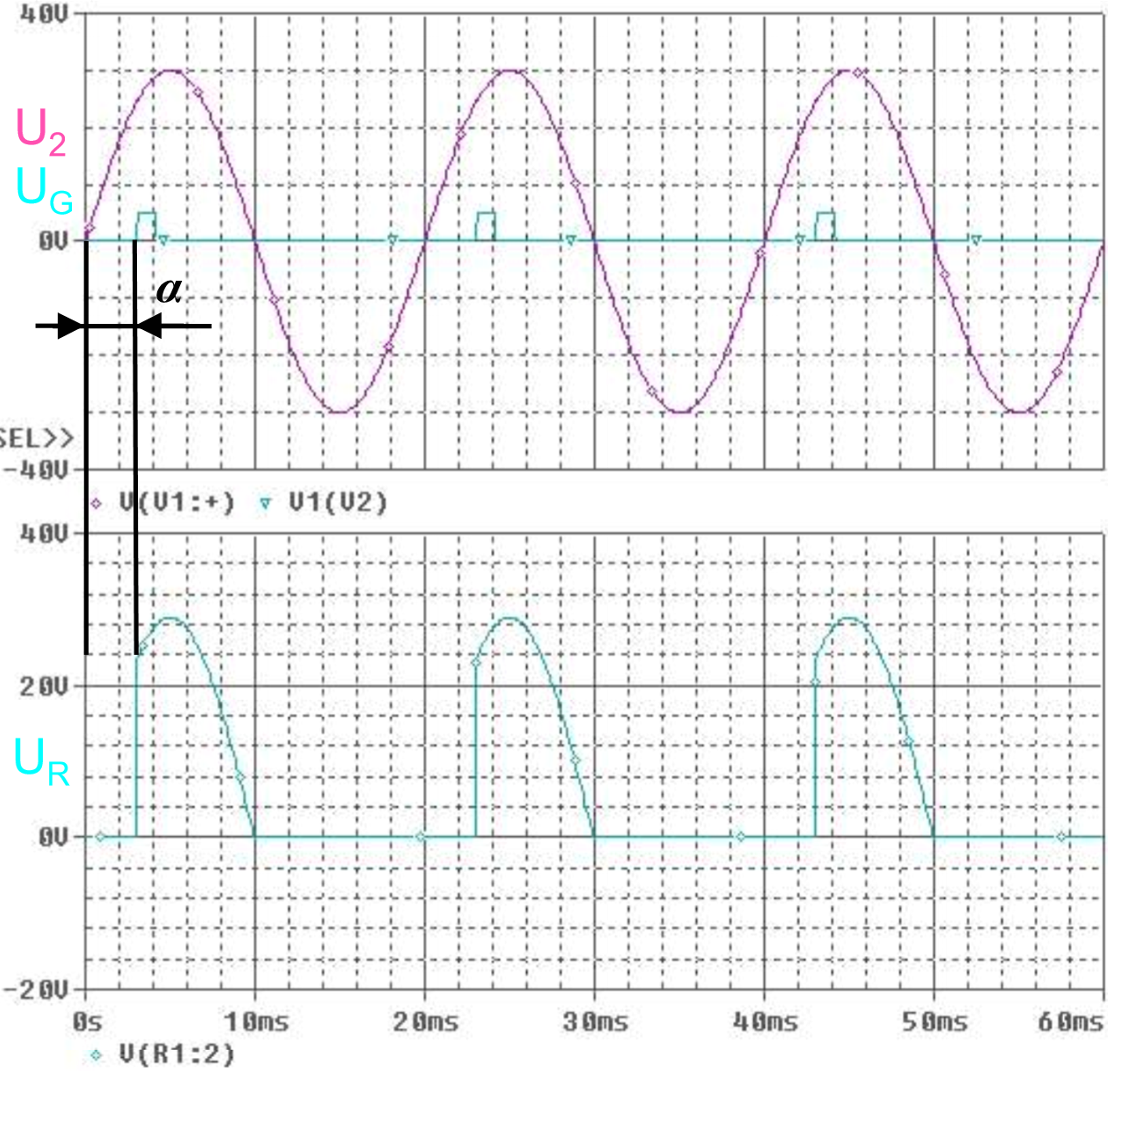
\includegraphics[width=0.8\linewidth]{images/M1CKl}

\end{minipage}
\begin{minipage}{0.25\linewidth}
    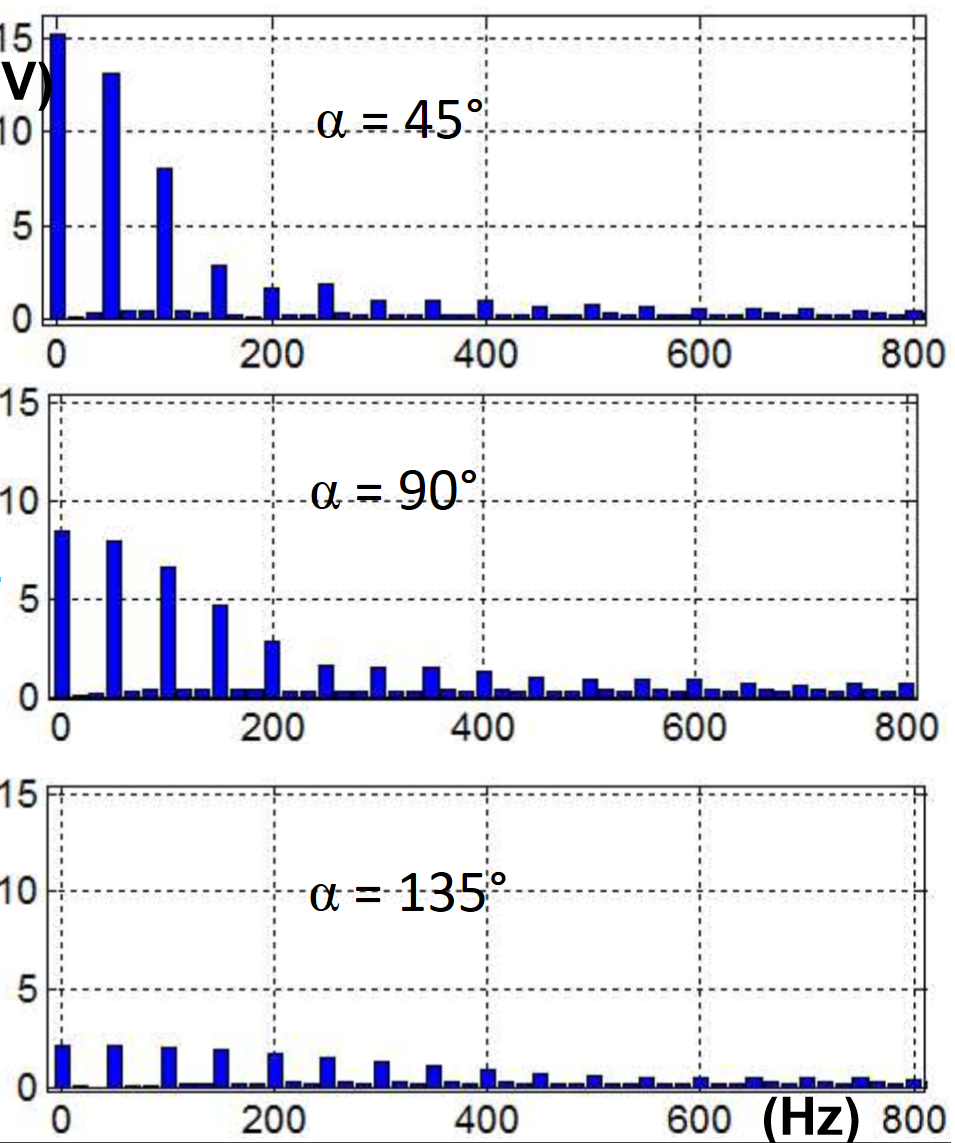
\includegraphics[width=0.8\linewidth]{images/M1COW} 
\end{minipage}
\newline
\vspace{-0.8cm}
\begin{longtable}{ p{.2\textwidth}  p{.50\textwidth}  p{.25\textwidth} } %TODO Formeln einfügen
    Mittelwert&
    $ \bar{U}_{OUT} = \dfrac{1}{2\pi} \int\limits_{\alpha}^{\pi}\hat{U}_2\cdot sin(\beta) \diff \beta =\dfrac{\hat{U}_2}{2\pi}(1+cos(\alpha)) $&
    \[ \beta = \omega t\]
    \\[-1cm]
    Effektivwert&
    $ U_{R\; RMS}= \sqrt{\frac{U_{2m}^2}{2\pi}\cdot \int\limits_{\alpha}^{\pi} sin(\beta)^2 \diff \beta}
    = U_{2m}\cdot \sqrt{\frac{\pi - \alpha}{4 \pi}+ \frac{sin(2\alpha)}{8\pi}}$&
    \\
\end{longtable}
\vspace{-0.5cm}

%===================================================================
%\clearpage

\subsection{B2C}
\begin{minipage}{0.4\linewidth}
    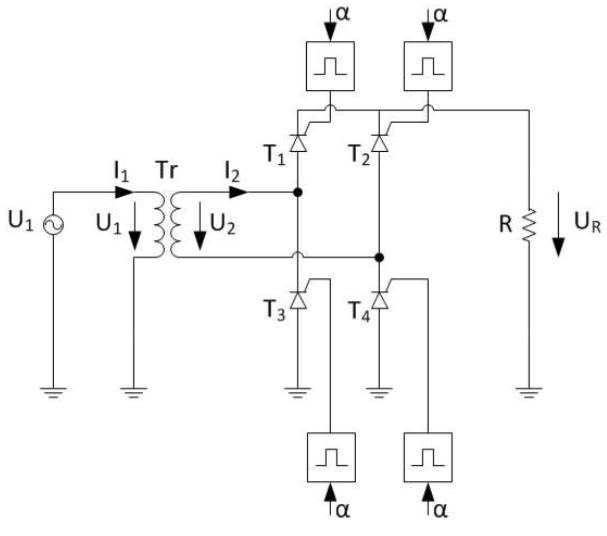
\includegraphics[width=0.8\linewidth]{images/GRB2c}
\end{minipage}
\begin{minipage}{0.35\linewidth}
    \centering 
    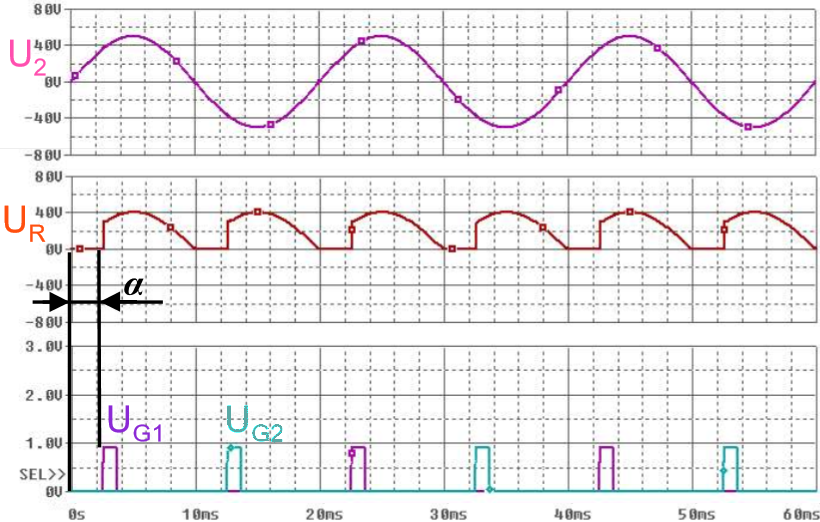
\includegraphics[width=0.8\linewidth]{images/B2CKl}
    
\end{minipage}
\begin{minipage}{0.25\linewidth}
 %TODO Oberwellengrafik 
   %\includegraphics[width=\linewidth]{images/B2COW} 
\end{minipage}
\newline
\vspace{-0.8cm}
\subsubsection{Rechnungsbeispiel}
\renewcommand{\arraystretch}{2}
\begin{tabular}{ p{.2\textwidth}  p{.50\textwidth}  p{.25\textwidth}}
    Mittelwert:&
    $ U_{R \;AV} = \frac{1}{\pi}\int\limits_{\alpha}^{\pi} U_{2m} \cdot sin(\beta)\diff \beta = \frac{U_{2m}}{\pi}(1+ cos(\alpha))$& $\beta = \omega t$
    \\
    Effektivwert: &
    $ U_{R \; RMS}=\sqrt{\frac{2 U_{2m}^2}{T}\cdot \int\limits_{\alpha}^{\nicefrac{T}{2}} sin(\frac{2\pi}{T}t)^2\diff t} \newline
    \hspace*{1cm} =\sqrt{\frac{U_{2m}^2}{\pi}\cdot \int\limits_{\alpha}^{\pi} sin(\beta)^2 \diff \beta}= U_{2m}\cdot \sqrt{\frac{\pi - \alpha}{2 \pi}+ \frac{sin(2\alpha)}{4\pi}}$&
    $ \beta = X \cdot t \rightarrow \diff \beta = X \cdot \diff t$
    \\
\end{tabular}
\renewcommand{\arraystretch}{1}
    \textbf{Übung 5 - Gesteuerte Gleichrichter B2C mit Fremderregte GSM}\newline
\hspace*{2cm}
\begin{minipage}{\linewidth}
    \textbf{Siehe FS ElMasch}\newline
    $\alpha$~=~Anschnitt-Winkel \hspace{2cm} $\beta$~=~Abschnitt-Winkel durch Induzierte Spg.
\end{minipage}
%===================================================================
%\clearpage
\vspace{-0.7cm}

\subsection{B6C}
\begin{minipage}{0.4\linewidth}
    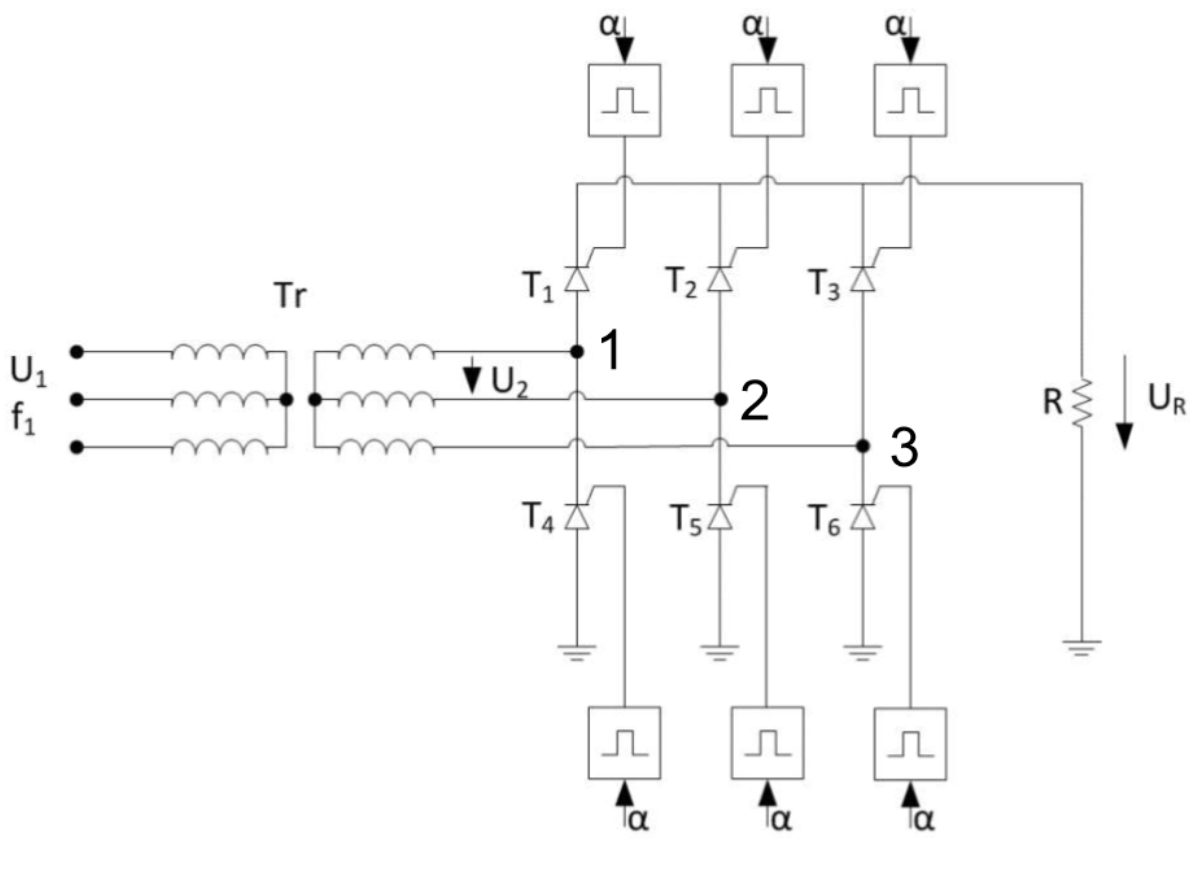
\includegraphics[width=0.8\linewidth]{images/GRB6c}
\end{minipage}
\begin{minipage}{0.35\linewidth}
    \centering 
    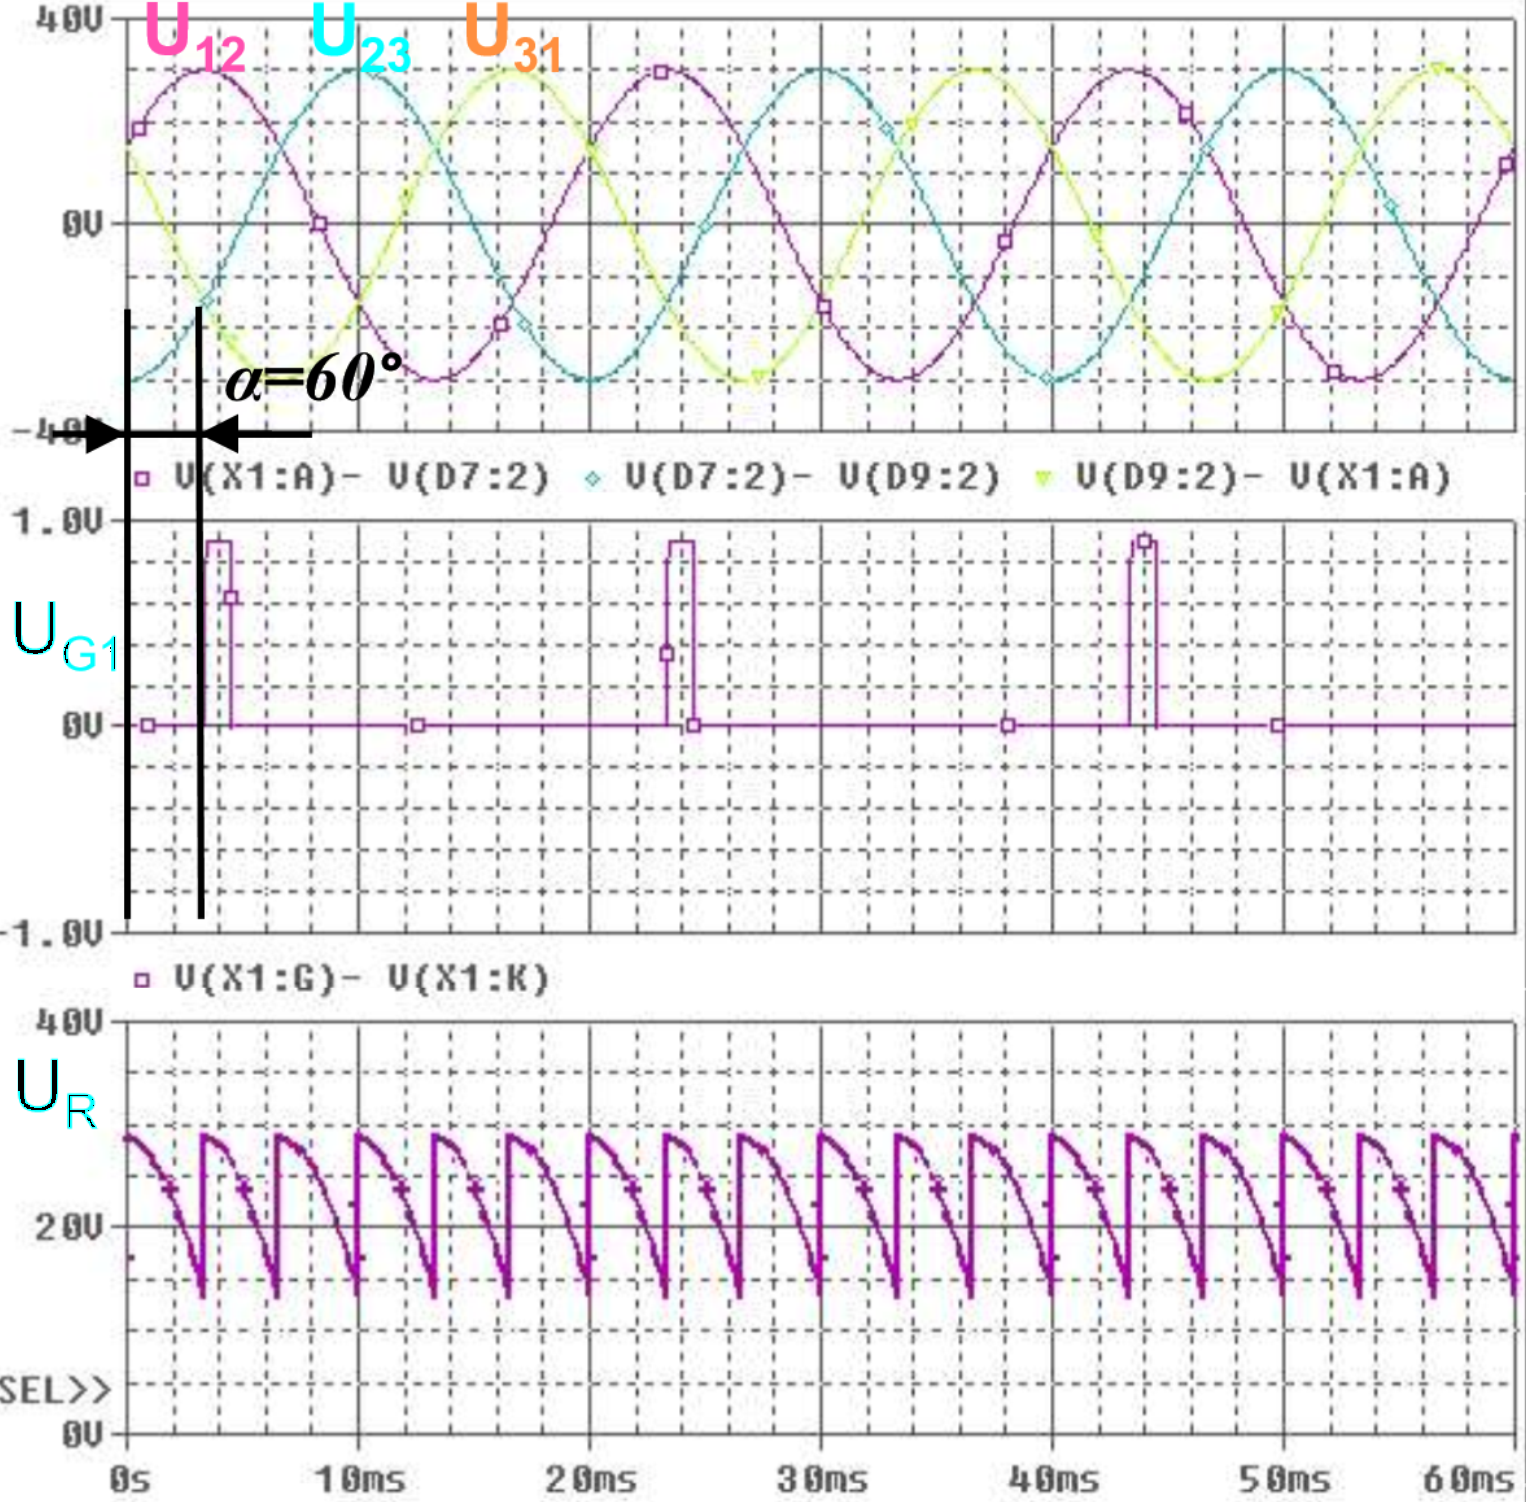
\includegraphics[width=0.8\linewidth]{images/B6CKl}
    
\end{minipage}
\begin{minipage}{0.25\linewidth}
  %TODO Oberwellengrafik 
  %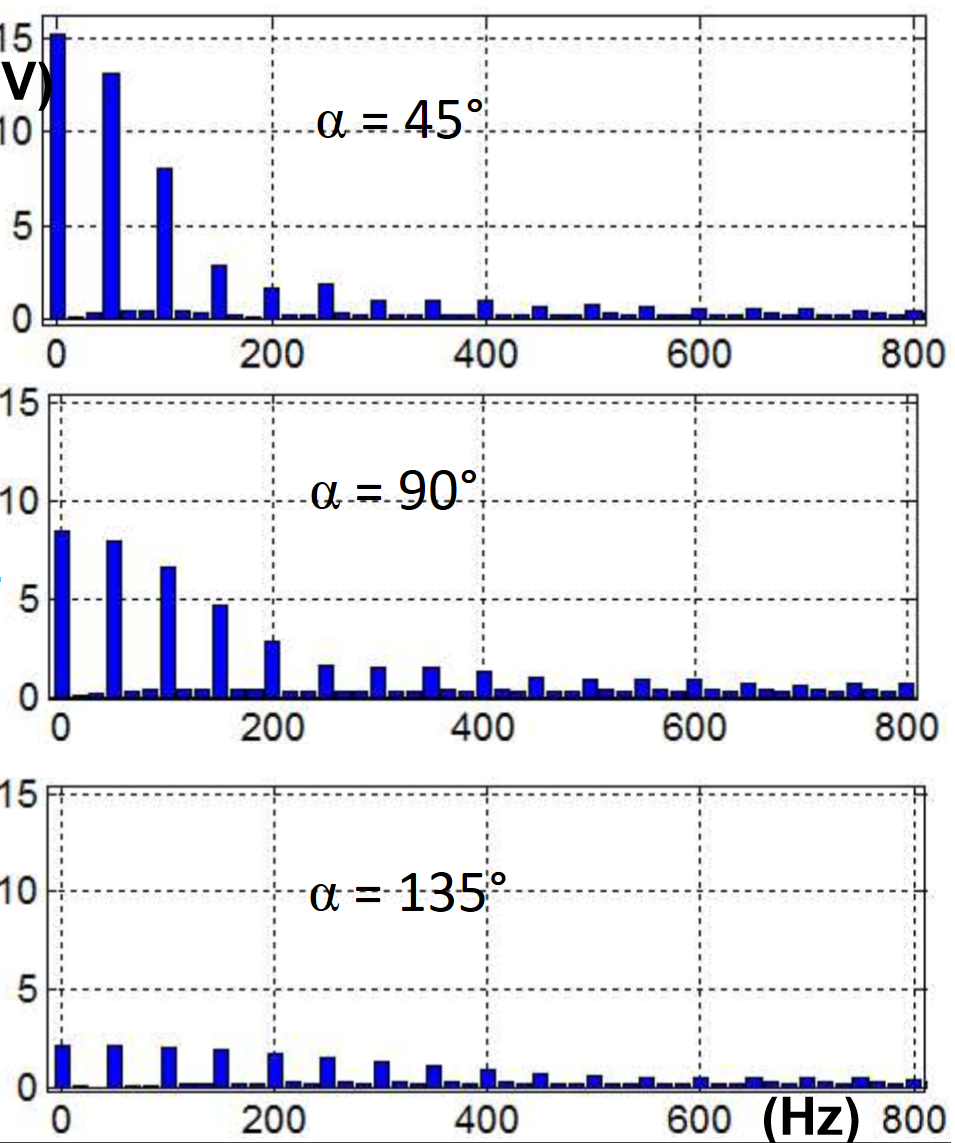
\includegraphics[width=\linewidth]{images/M1COW} 
\end{minipage}
\newline

%===================================================================
\clearpage